%% source: 2023-sp-midterm_02
%% tags: [bellman-ford]
\begin{prob}

    Recall that the outer loop of the Bellman-Ford algorithm \textit{without}
    early stopping loops for a fixed number of iterations, while the inner loop
    iterates over each edge of the graph.

    Suppose Bellman-Ford \textit{with} early stopping is run on the graph below using node
    $s$ as the source:

    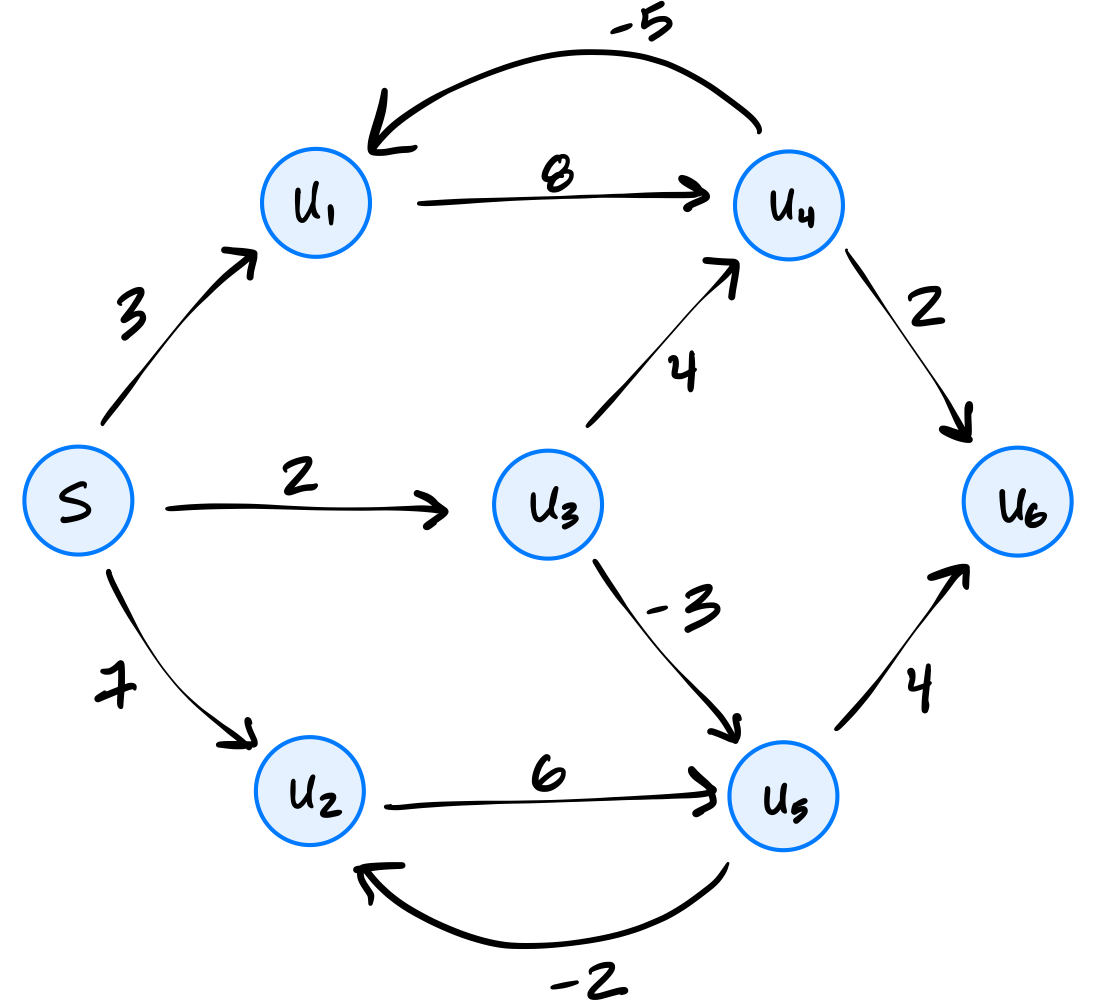
\includegraphics{./graph.png}

    What is the fewest number of iterations of the outer loop that can possibly
    be performed?

    \begin{soln}
        2
    \end{soln}

\end{prob}
